\clearpage

\subsection{Testen}
\label{sec:Testen}

\subsubsection{Klassifizierung von Testverfahren}
\label{sec:KlassifizierungTestverfahren}

\begin{multicols}{2}
	\begin{itemize}
		\item Wer testet?
		\begin{itemize}
			\item Mensch (manuell) vs. Maschine (automatisch)
			\item Entwickler vs. Benutzer
		\end{itemize}
		\item Was wird getestet?
		\begin{itemize}
			\item Komponente (Unit-Test/Funktionstest/Klassentest) vs. Integration vs. System (End-to-End)
			\item Testpyramide
		\end{itemize}
		\item Wie wird getestet?
		\begin{itemize}
			\item Bottom-Up vs. Top-Down
			\item statisch (Kompilierzeit) vs. dynamisch (Laufzeit)
			\item ohne Kenntnis des Codes (Blackbox) vs. mit Kenntnis des Codes (Whitebox)
			\item explorativ
			\item Schreibtischtest/Review
		\end{itemize}
		\item Wann wird getestet?
		\begin{itemize}
			\item Vor vs. nach der Entwicklung
			\item Abnahmetest
		\end{itemize}
		\item Warum wird getestet?
		\begin{itemize}
			\item Regressionstest
			\item Lasttest/Belastungstest
			\item Smoketest
		\end{itemize}
	\end{itemize}
\end{multicols}
\begin{center}
	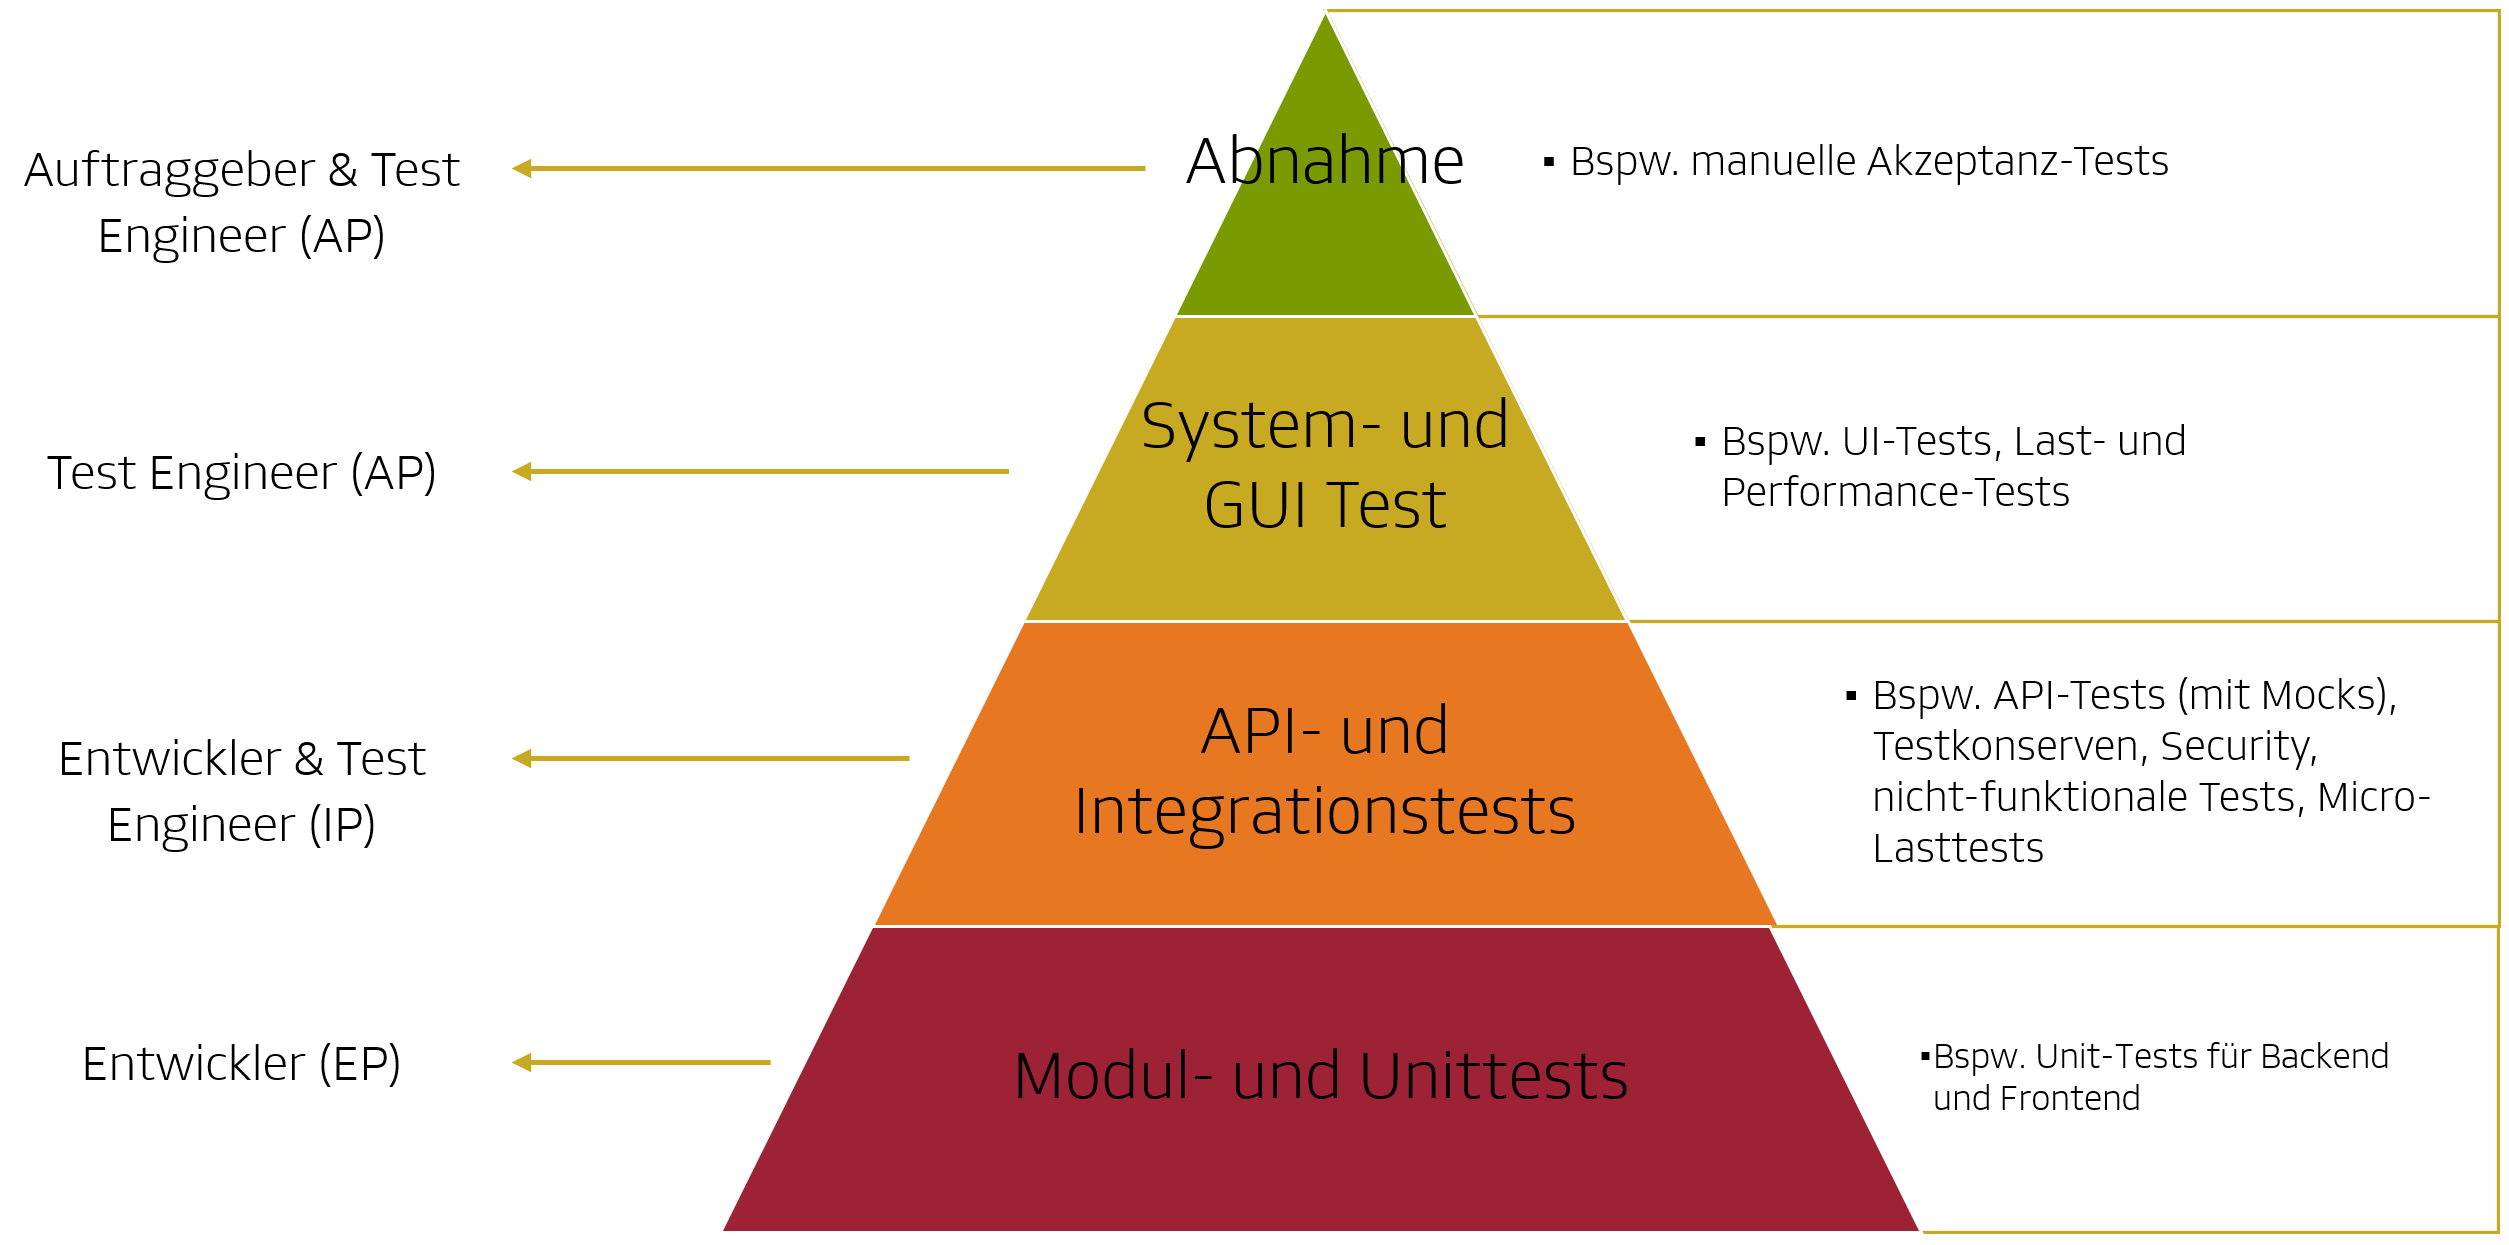
\includegraphics[scale=.4]{Bilder/testpyramide.png}
	\textbf{Testpyramide:} Quelle: dvag \cite{Testpyramide}
\end{center}

\begin{center}
	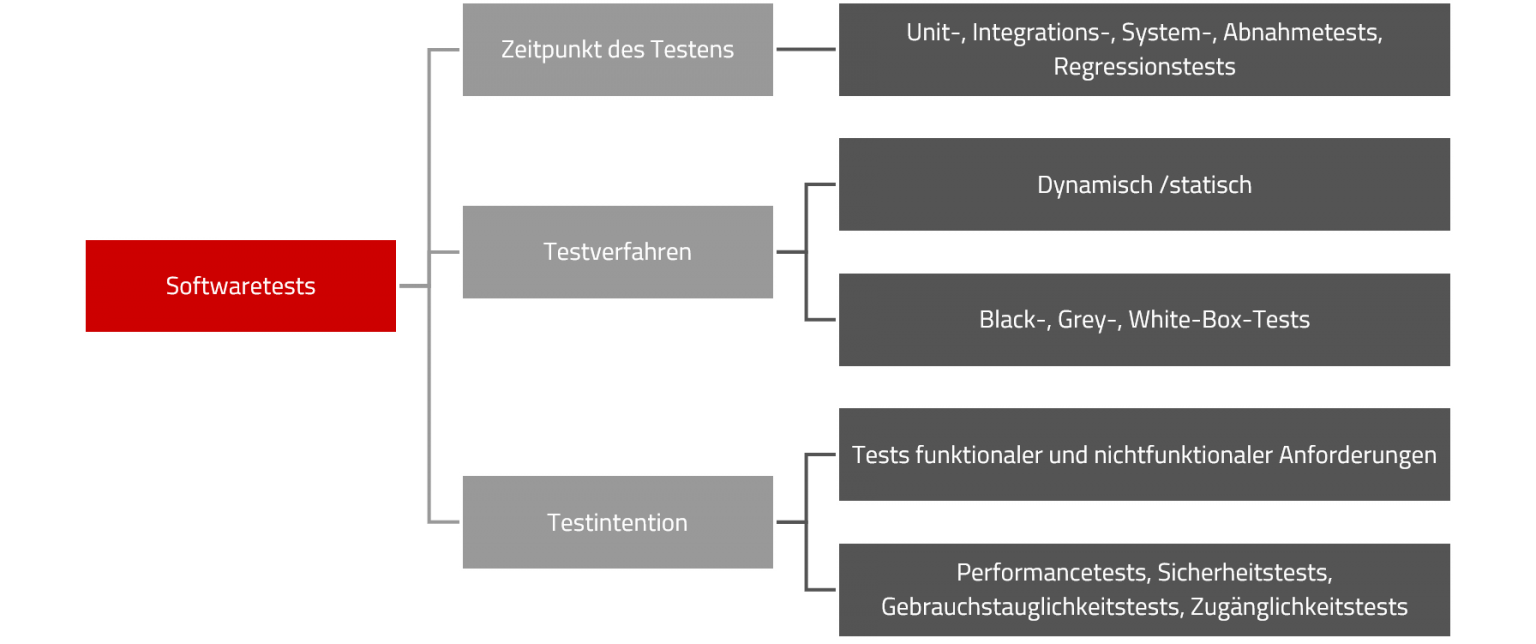
\includegraphics[scale=.32]{Bilder/TestsKlassifizierung.png}
	Quelle: redbots \cite{testKlassifizierung}
\end{center}

\clearpage

\textbf{Top-Down}
\begin{itemize}
	\item \textbf{Definition:} Beim Top-Down-Testen beginnt das Testen auf der höchsten Ebene der Softwarehierarchie und bewegt sich allmählich zu den unteren Ebenen. Das bedeutet. dass das Testen mit den breiteren Funktionalitäten des Systems beginnt und dann in feinere Details eindringt.
	\item \textbf{Prozess:} Der Testprozess beginnt mit dem Testen der Hauptmodule der Software und bewegt sich dann allmählich zum Testen kleinerer Teilmodule und einzelner Einheiten.
	\item \textbf{Vorteile:}
	\begin{itemize}
		\item Frühes Erkennen von Problemen auf hoher Ebene oder architektonischen Mängeln.
		\item Ermöglicht das Testen kritischer Funktionalitäten und Benutzerinteraktionen zuerst.
		\item Kann schnelles Feedback zum Gesamtverhalten des Systems liefern.
	\end{itemize}
	\item \textbf{Nachteile:}
	\begin{itemize}
		\item Probleme auf niedrigerer Ebene können bis zu späteren Phasen unentdeckt bleiben.
		\item Abhängigkeiten von Modulen auf niedrigerer Ebene können zu Verzögerungen beim Testen führen.
		\item Möglicherweise sind Stub-Objekte oder Mock-Objekte für unvollständige oder untergeordnete Module erforderlich.
	\end{itemize}
\end{itemize}

\textbf{Bottom-Up}
\begin{itemize}
	\item \textbf{Definition:} Beim Bottom-up-Testen beginnt der Testprozess auf der untersten Ebene der Software-Hierarchie und bewegt sich nach oben. Es beginnt mit der Prüfung einzelner Einheiten oder Module und integriert sie dann schrittweise, um größere Komponenten zu testen.
	\item \textbf{Prozess:} Der Testprozess beginnt mit der Prüfung der kleinsten Codeeinheiten (wie Funktionen oder Methoden) und geht dann zur Prüfung größerer Komponenten über, indem diese Einheiten integriert werden.
	\item \textbf{Vorteile:}
	\begin{itemize}
		\item Früher Nachweis von Problemen auf Codeebene.
		\item Ermöglicht gründliche Tests einzelner Einheiten in Isolation.
		\item Ermöglicht die frühe Identifizierung von Integrationsproblemen.
	\end{itemize}
	\item \textbf{Nachteile:}
	\begin{itemize}
		\item Probleme auf höherer Ebene können erst in späteren Phasen entdeckt werden.
		\item Die Integrationsprüfung kann verzögert werden, bis alle Einheiten getestet sind.
		\item Erfordert eine sorgfältige Planung, um höhere Funktionalitäten für die Prüfung isolierter Einheiten zu simulieren.
	\end{itemize}
\end{itemize}